% Figure 2: 6-Layer Stack Architecture
% Design Spec: docs/era-smartfarm-rag/paper/figures/6_LAYER_STACK_DESIGN_SPEC.md
% TODO: Replace with actual TikZ diagram implementing 6-layer vertical stack

\begin{figure}[htbp]
\centering
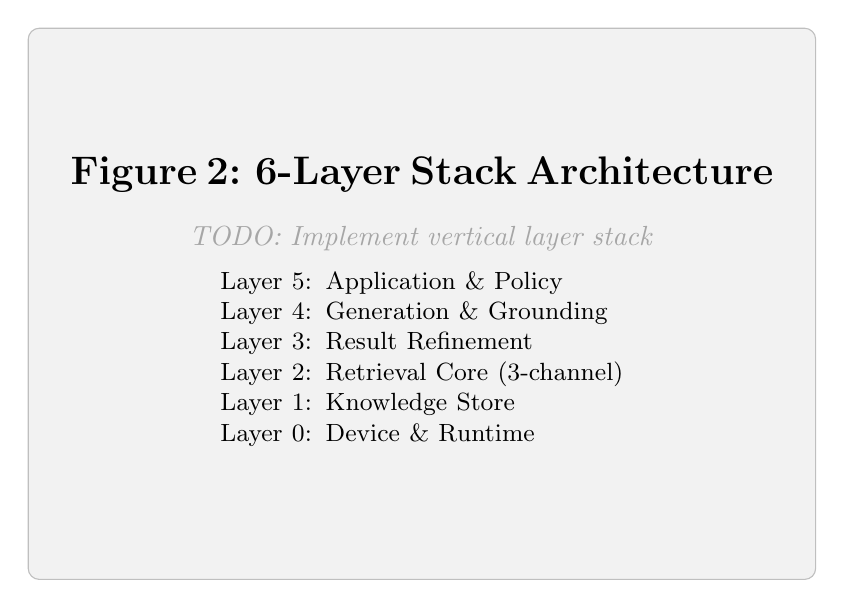
\begin{tikzpicture}
  \node[rectangle, draw=gray!50, fill=gray!10, minimum width=10cm, minimum height=7cm, rounded corners] (placeholder) {};
  \node[text width=9cm, align=center] at (placeholder.center) {
    \textbf{\Large Figure 2: 6-Layer Stack Architecture}\\[1em]
    \textcolor{gray!70}{\textit{TODO: Implement vertical layer stack}}\\[0.5em]
    \small
    \begin{tabular}{l}
    Layer 5: Application \& Policy \\
    Layer 4: Generation \& Grounding \\
    Layer 3: Result Refinement \\
    Layer 2: Retrieval Core (3-channel) \\
    Layer 1: Knowledge Store \\
    Layer 0: Device \& Runtime \\
    \end{tabular}
  };
\end{tikzpicture}
\caption{Edge RAG 6-layer architecture with hardware constraints (Layer 0), knowledge storage (Layer 1), hybrid retrieval core (Layer 2), result refinement (Layer 3), generation (Layer 4), and application layer (Layer 5).}
\label{fig:layer-stack}
\end{figure}
